\documentclass[12pt]{article}

\usepackage{cls}
\usepackage{tipa}
\usepackage{enumerate}
\title{Resistance to phonetic change in York, Northern England}
\author{Daniel Lawrence}
\organization{The University of Edinburgh}

\begin{document}

\maketitle

\section{Introduction}
This paper reports on a sound change in progress in York, Northern England. The change in question involves the fronting of the tense back vowels \textipa{/u/} and \textipa{/o/}, which is of particular interest due to its prevalence across varieties of English. This change has been documented in North America (Baranowski, 2008; Hall-Lew, 2009), Australia (Cox, 1999), New Zealand (Easton \& Bauer, 2000) and in the United Kingdom (Kerswill \& Williams, 2005), as well as in typologically-unrelated languages (e.g. Swedish, Proto-Southern Yiddish, Albanian, Akha; see Labov (1994)). Surveying previous work reveals a number of generalizations regarding the phonological patterning of these changes and their relationship:


\begin{enumerate}
\item{Back vowel fronting involves the generalization of synchronic fronting processes across phonetic environments.}
\item{\textipa{/o/ fronting typically only occurs in dialects where there is evidence of /u/ fronting.}}
\item{In varieties where both vowels are fronting, the nucleus of \textipa{/u/} remains more advanced in F2 space than that of \textipa{/o/}.}
\end{enumerate}

The first of these generalizations refers to the fact that back vowels are fronted in post-alveolar contexts as a consequence of consonant-on-vowel coarticulation. Change in these vowels tends to involve productions in non-fronting contexts moving forward, while productions in conditioning environments remain relatively constant. This pattern, reported in e.g. Durian, (2014); Harrington et al., (2006) and Hall-Lew (2011), can be taken as evidence of a process of perceptual reanalysis, where learners' failure to compensate for coarticulation leads to their production targets shifting toward highly-frequent coarticulatory allophones (Ohala, 1993). 

The second generalization was first noted in Labov, Ash and Boberg (2005). Surveying the relationship between /o/ and /u/ fronting In North America, they demonstrate that North American dialects of English can be divided into three groups -- those that front /u/ alone, those that front both /u/ and /o/, and those that front neither. In no cases do they find a variety where /o/ fronts in the absence of /u/. In principle, such a pattern could arise simply due to historical accident -- if /u/ fronting began first, followed independently by /o/ fronting, then it would still be possible to observe this apparent implication relationship between the two vowels. However, the third generalization listed above suggests otherwise -- there appears to be a bias toward maintaining preserving the phonetic relationship between the two vowels, whereby the nucleus of /o/ never advances beyond that of /u/. This evidence has lead to the proposal that change in /o/ and /u/ is a parallel shift, either driven by pressures toward preserving symmetry in the vowel space (Martinet, 1952), or due to the vowels' shared membership in a phonological class (Fruehwald, 2013).

While these patterns are well-attested for North American dialects, and to some extent in RP (Harrington, 2007, 2008), there is some debate as to whether northern dialects of British English are exceptional with regard to these patterns. For example, it has been claimed that \textipa{/o/} fronting occurs in the absence of \textipa{/u/} fronting in Bradford, West Yorkshire (Watt \& Tillotson, 2001). A potential reason for this might be related to dynamic properties of the back vowels in these dialects -- the variable diphthongization of \text{/o/} is widely cited as a key shibboleth of Northern/Southern regional identity in Britain. Since the interaction of fronting and diphthongization may produce a wide range of realizational possiblities for these vowels, it is reasonable to hypothesize that dynamic properties of \textipa{/o/} and \textipa{/u/} may play a role in the sociolinguistic distribution of this change, resulting in outcomes which contrast patterns identified in other varieties. In light of this, the present study presents evidence for ongoing back vowel fronting in the northern English city of York. In doing so, it seeks to answer the following questions:

\begin{enumerate}
\item{To what extent does the fronting of \textipa{/o/} and \textipa{/u/} in this community reflect previous generalizations regarding back vowel fronting?}
\item{How do dynamic properties of \textipa{/o/} and \textipa{/o/} influence the sociolinguistic trajectory of these changes?}
\end{enumerate}

\section{Data \& Methods}

\subsection{Data}

Data are taken from a corpus of production data collected from 52 individuals born between 1930 and 2000. Speakers were recruited using convenience sampling, as is typical in variationist sociolinguistic work. Table 1 provides the speakers' basic demographic information.

\vspace*{6pt}
\begin{table}[htbp]
\centering
\begin{tabular}{l|l|l}
Birth year&Female & Male \\
1935-1960 &7 &5\\
 1961-1980& 8 & 11\\
1981-2000& 10 &11\\
\end{tabular}
\caption{Characteristics of the speaker sample}
\end{table}
\vspace*{6pt}

The data include a) a 100-item wordlist, including 15 tokens of each vowel in a range of phonetic environments plus fillers; b) a map task (Anderson et al., 1991) using a selection of words from the word list and c) a sociolinguistic interview, including a range of questions relevant to the speakers' social background and identity with regard to York and the north of England. 

\subsection{Measurement}

Vowels were segmented from the first to the last glottal pulse visible in the spectrogram, and measurements of F1, F2 and F3 were taken at 20 equidistant points along the vowel trajectory. The present analysis will focus on F2 trajectories, which provide a relatively reliable reflection of the degree of fronting. Measurements were normalized using the modified Watt \& Fabricius normalization method (Watt \& Fabricius, 2002), using the mean midpoint values of \textipa{/A/} and \textsc{/i/}, measured from 4 tokens per vowel per speaker, as reference points. The formant values provided in the present analyses are of the form $F^n/S (F^n)$, i.e. the ratio of the measured frequency in Hz to the centroid frequency of that formant for the speaker being analyzed.

\subsection{Statistical analysis}

Typical sociophonetic studies have relied on the analysis of single points of the vowel trajectory (either at a fixed percentage of the token, or based on the analyst's identification of a `steady-state' target), or summary measures of trajectory length (e.g. ). The limitation of these approaches is that they may miss crucial aspects of fine-grained temporal variation in vowel realizations. In order to avoid these pitfalls, the results presented in the following sections use the statistical technique of \textit{Generalized Additive Modeling}, which allow vowel tokens to be summarized as smooth functions of time. Winter \& Wieling (2016) give a concise summary of the application of such models to time-varying linguistic data. Their key relevance of such models to the present study is that they allow the analyst to capture potentially non-linear changes in the dynamic properties of vowels, without enforcing any apriori assumptions about the shape of vowel trajectory and trajectory of change. The models presented in this paper predict normalized F2 as a function of time, plus the variables listed below:

\vspace*{6pt}
\begin{table}[htbp]
\centering
\begin{tabular}{l|l|}
Variable&Form \\
Phonetic environment &/o/: ow owN Tow Jow\\& /u/: Juw Tuw Kuw uwL \\
Log duration& Continuous \\
Speaker year of birth& Continuous (1935-2000)\\
Speaker gender& M/F \\
Speaker level of education & 1=Secondary only\\& 2=Higher education\\&3=Postgraduate/\\&professional training\\
\end{tabular}
\caption{Variables tested}
\end{table}
\vspace*{6pt}
The baseline models included constant terms for linguistic factors and their smooth interactions with time. Random smooths were included for each speaker, allowing the model to account for individual variation in vowel production.
The influence of non-linguistic factors was tested by performing a Chi-square test on models including those factors and ones with only linguistic factors. The results of the analysis are presented below:

[Table 3: model selection]

\section{Evidence of \textipa{/o/} and \textipa{/u/} fronting in York}
Figure 1 visualizes the main effect of speaker year of birth on the second formant of \textipa{/o/} and \textipa{/u/}. At this stage, the analysis will focus on estimates taken at the vowel midpoint (50\%) -- see section 6 for a detailed discussion of the role of dynamic variation. The results demonstrate that the F2 midpoint of both vowels is reliably higher with increasing speaker year of birth, providing apparent-time evidence that both vowels have undergone fronting over the past $~$60 years. Change in \textipa{/u/} appears to have proceeded in a slightly more regular fashion that change in \textipa{/o/}, evidenced in the slightly tighter clustering of speaker means around the model predictions in Figure 1 -- a model including linguistic factors and speaker year of birth explains 57\% of the variation in /u/ F2, but only 23\% of variation in /o/. The smooth functions estimated by the GAM analysis are roughly s-shaped, consistent with established findings on the temporal dynamics of linguistic change (e.g. Labov, xxxx). Having presented evidence of \textipa{/u/} and \textipa{/o/} fronting in this variety, the following section will explore the extent to which this change conforms to previous generalizations regarding back vowel fronting.
\begin{figure}[!htbp]
\centering
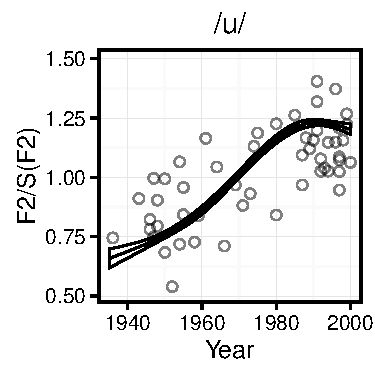
\includegraphics{uwchange}
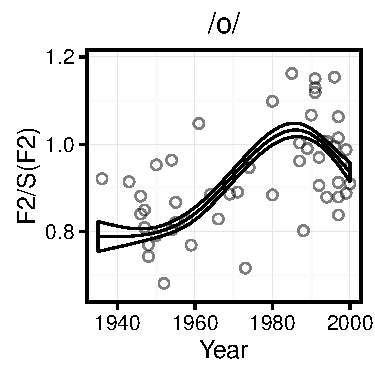
\includegraphics{owchange}
\caption{Evidence of \textipa{/o/} and \textipa{/u/} fronting}
\end{figure}

\section{The coarticulatory basis of \textipa{/u/} and \textipa{/o/} fronting}

Figure x demonstrates the role of coarticulation in conditioning back vowel fronting in this variety. In both cases, a pattern of co-articulatory variation is present at the onset of the change, which reduces as the change progresses. This pattern is most noticable in the case of /u/ (left panel). For the oldest speakers in the sample, /u/ is produced with a phonetically fronted variant following a palatal or coronal consonant (e.g. in \textit{june} and \textit{two}), and with a back variant in all other contexts. The change takes place primarily in the non-phonetically fronting contexts, meaning that the youngest speakers in the sample produce forms such as \textit{food} and \text{noon} with the fronted variant which was previously restricted to postcoronal and postpalatal environments. A similar, but less striking pattern is evident in /o/: the difference between phonetically conditioning and non-conditioning environments is much smaller among the youngest speakers in the sample, suggesting that change in this vowel involves the effect of coarticulation decreasing over time. The data for /u/ also provide evidence of the early phonologization of back pre-/l/ environments (c.f. Fruehwald, 2013), which are reliably distinct from the other environments at the earliest stages in the change, and show no evidence of fronting.

Taken together, these results demonstrate that back vowel fronting in York adheres to the first generalization discussed in the introduction of this paper. As has been reported in other varieties of English, the coarticulatory fronting of /u/ and /o/ appears to provide a source for diachronic change, evidenced in the weakening of the coarticulatory effects on these vowels as these changes progress.  
\begin{figure}[!htbp]
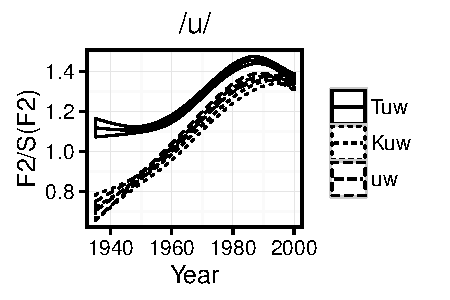
\includegraphics{uwphoneticconditioning}
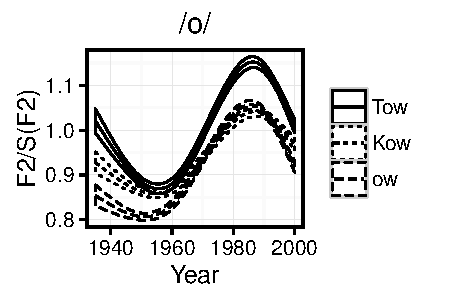
\includegraphics{owphoneticconditioning}
\caption{Changes in the phonetic conditioning of /o/ and /u/ fronting.}
\end{figure}

\section{\textipa{/o/} and \textipa{/u/} fronting as a parallel shift}

The second and third generalization listed in the introduction concerns the relationship between the two vowels when undergoing change. /o/ fronting seems to occur only in dialects where there is also evidence of /u/ fronting, suggesting an implicational relationship between change in the two vowels. This pattern is demonstrated in Labov et al. (2005), who find that American dialects can be grouped into three categories based on their typical realizations of /o/ and /u/: those which show no evidence of either /o/ or /u/ fronting; those which show evidence of /u/ fronting only, and those which show evidence of both /o/ and /u/ fronting. This pattern is schematized in Figure x, adapted from Labov et al. (2005:143).
  
\begin{figure}[!htbp]
\centering
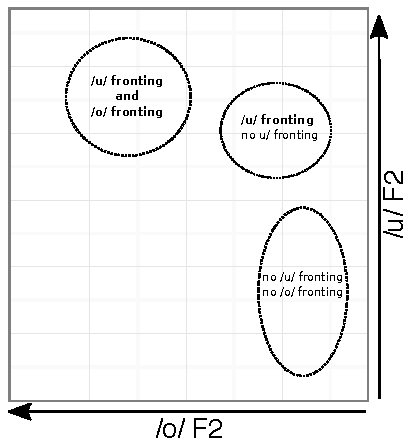
\includegraphics[scale=0.8]{owuwANAE.pdf}
\caption{The relationship between /o/ and /u/ in North American dialects of English.}
\end{figure}

Given the evidence of the fronting of both /u/ and /o/ fronting presented in section 3, it is clear that York conforms to this pattern. However, exactly what causes this pattern is still an open question. There are at least two possible explanations:
\begin{enumerate}[(a)]
\item{historical accident -- change in /o/ and /u/ could have begun independently and diffused across these sets of dialects, with the apparent implicational relationship arising simply because change in /u/ occurred before change in /o/.}
\item{the fronting of /u/ could be a trigger for the fronting of /o/, freeing up the back of the vowel space and initiating a chain shift (but not in all dialects)}
\end{enumerate}
There are two pieces of evidence which shed light on this question. Firstly, it appears that /u/ fronting did precede /o/ fronting in this community. Figure 4 plots the estimates for the trajectories of change for both vowels. The left hand panel shows the model predictions for the mean F2 for each year, while the right-hand panel shows the first derivative of those curves, providing an estimate of the rate of change. From these plots it can be inferred that /u/ fronting was already in progress as early as 1940, and reached its peak around 1970, before slowing down and reaching completion in the 1990s. Change in /o/ began around 20 years after change in /u/, visible where the /o/ curve crosses zero in the right-hand panel. Similar to /u/, change in /o/ reached its peak around 1970, then slowed down before reaching completion in the 1990s. Although /u/ begins to front before /o/, it is notable that after change in /o/ initiates, the two vowels seem to front at nearly same rate, reach a peak at the same time, and begin to reverse together. The fact that the two vowels show such strikingly similar trajectories of change suggests that there is a robust internal relationship between them.
\begin{figure}
\centering
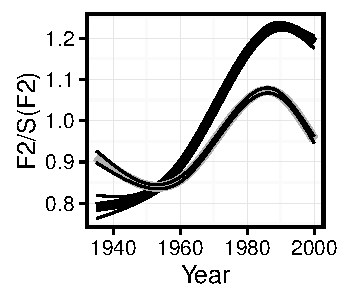
\includegraphics{owuwparallel.pdf}
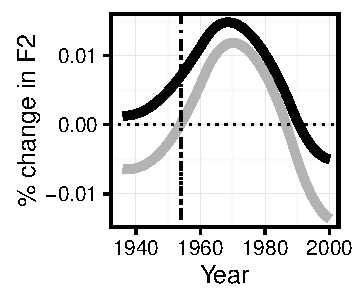
\includegraphics{owuwparallelROC.pdf}
\caption{The temporal relationship of /o/ and /u/ fronting.}
\end{figure}

\subsection{Within-speaker relationship}
\begin{figure}
\centering
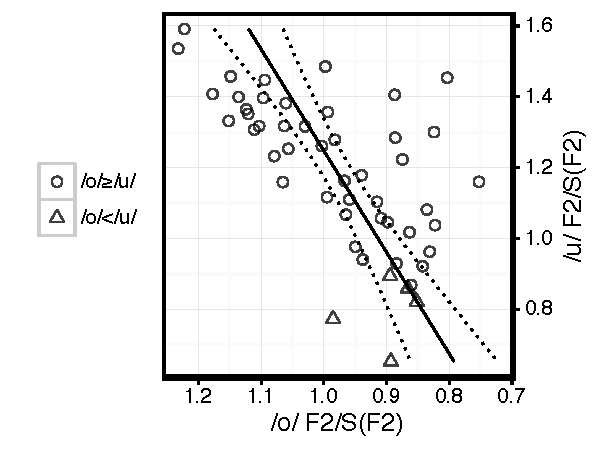
\includegraphics{owuwcorrelation.pdf}
\caption{Within-speaker relationship between /o/ and /u/.}
\end{figure}
Figure 5 demonstrates a robust correlation between individual speakers' degree of fronting in /o/ and /u/. The nature of this correlation is interesting in two ways -- firstly, the data is not normally distributed around the regression line; rather, they are skewed towards the lower values of /o/ F2. This reflects a conditional relationship between the two vowels -- there is evidence of speakers with back /o/ and back /u/ (in the bottom, right-hand corner of the plot); those with back /o/ and fronted /u/ (top, right-hand corner of the plot), and those who front both /o/ and /u/ (top, left-hand corner of the plot). The second important observation is that the relationship between /o/ and /u/ is maintained at the level of the individual speaker -- individuals appear to maintain a relationship between the two vowels such that the nucleus of /o/ remains more retracted in F2 space than that of /u/. In only three cases (represented by triangles above) do speakers show evidence of an /o/ nucleus equal to or in advance of /u/.

\section{The role of vowel dynamics}
To summarize the evidence presented so far, the data provide robust evidence of the fronting of /o/ and /u/ over the past 60 years. Change in these vowels is consistent with previous accounts of similar changes across varieties of English, in a number of ways:

\begin{itemize}
\item{The source of diachronic fronting appears to be related to synchronic consonant-on-vowel coarticulation, the effects of which decrease over time.}
\item{/u/ fronting precedes /o/ fronting temporally}
\item{/o/ fronting is conditional on /u/ fronting, that is, no speaker participates in /o/ fronting without having first fronted /u/.}
\end{itemize}

Taken together, this provides evidence of a chain-shifting system consistent with Labov's `Principle III' (Labov, 1994). It could be speculated that the reanalysis of coarticulatory variation provided the source for change in /u/, leaving a gap at the back periphery of the vowel space and motivating the subsequent fronting of /o/. Assuming that there is an internal pressure in favour of /o/ fronting, what remains to be explained is why some speakers appear to resist this pressure, fronting /u/, but retaining a back /o/ variant. Considering the dynamic patterns of these vowels and their social embedding may provide the answer.

\begin{figure}
\centering
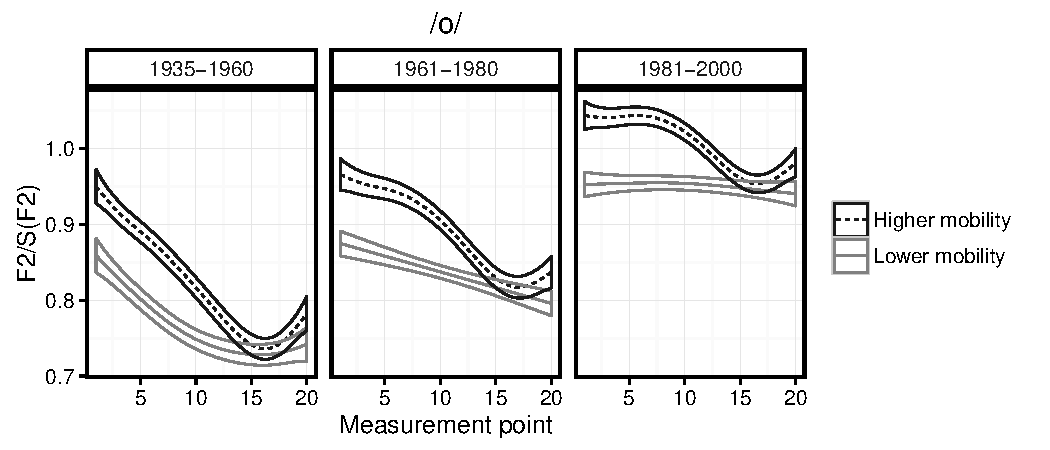
\includegraphics[scale=0.9]{owdynamicsclass.pdf}
\caption{Estimated /o/ F2 trajectory by decade and mobility group.}
\end{figure}


\begin{figure}
\centering
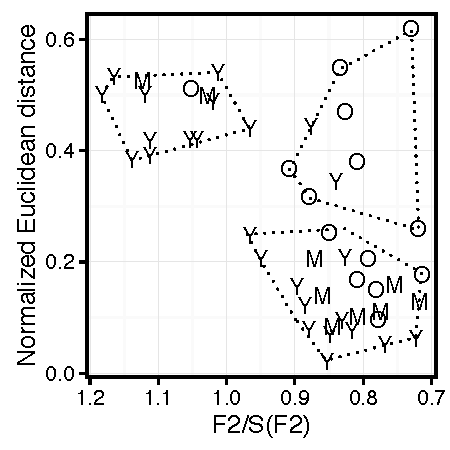
\includegraphics[scale=0.9]{ofrontingdip.pdf}
\caption{Relationship between /o/ fronting and diphthongization.}
\end{figure}

\section{Evaluating a sociolinguistic explanation}


\subsection{References}

Please use LSA style: name (year or (Name year). Formulations
with author names like ``\ldots\ as \namecite{Ladefoged:2003}
showed that \ldots'' are acceptable, but not ``as shown in [Ladefoged,
2003]'' or ``as shown in (Ladefoged~[6])''. See Section 4 for more on references.


\section{Format of references}

Monographs such as \namecite{Fant:1960} consist of author(s) last name(s),
initial of the first name(s), year of publication, title in italics, location of the publication, and publisher. The names of multiple authors are separated by commas listed in the 
sequence last name, comma, initial(s) of the first name(s) (cf.\ the examples~\citeboth{Beattie/etal:1982}, \citeboth{Peterson/Barney:1952}). 

Contributions to volumes, e.g.~\namecite{Stevens:1999}, follow the
convention that the title of the volume is in italics, but not the
title of the contribution. Book editors should appear after the book title, 
followed by page numbers, place of publication, and publisher.

Journal articles should be handled in the same way as contributions to
volumes, except that the title of the journal is in italics and
the editors are not listed. Longer names of well-known journals can be
abbreviated (e.g.~\citeboth{Peterson/Barney:1952}).

Articles in conference proceedings such as \namecite{Ladefoged:2003} are
referenced in the same way as journal articles.  The word
\textit{proceedings} can be abbreviated and the location should be
mentioned after the name of the conference. Here, abbreviations of
well-known conferences are possible.

\bibliographystyle{clslike}
\bibliography{cls}

\end{document}

